\section{Drift in a published irreversibility indicator}\label{sec:stommel}

Kooloth \textit{et al.}~\cite{kooloth2026} propose the lag-averaged difference between forward and backward cross-correlations of two state variables as an early warning of tipping, and illustrate it on a Stommel box model of the overturning circulation whose freshwater forcing $\eta_2=1.5\times10^{-3}\,t$ is ramped through a saddle-node. The estimator uses uncentered temperature $T$ and salinity $S$ in windows of $100$ time units, averages lags from $0.05$ to $4.95$ time units, and reports the ensemble mean of the absolute value. We regenerated the ensemble with the generation code included in the authors' notebook~\cite{koolothcode2025}, adding only seeds ($500$ realizations, the same stochastic integrator), and split the signed statistic exactly into a mean-path term, a fluctuation term and two cross terms whose ensemble mean vanishes, using the leave-one-out ensemble mean.

The mean-path term accounts for \MPshareMin--\MPshareMax\% of the signal at the four reporting times of the original figure; the fluctuation term is \FLshareMin--\FLshareMax\% of it and of opposite sign [Fig.~\ref{fig:stommel}(a)]. The statistic computed on the noise-free trajectory differs from the stochastic ensemble by at most \DetDiffMax\%; doubling the ramp rate at matched forcing multiplies it by \EpsRatioMin--\EpsRatioMax; and shifting the origin of temperature by one unit changes it by \OriginMin--\OriginMax\% [Fig.~\ref{fig:stommel}(b)]. The signal is therefore the drift of the mean state, which accelerates as the stable branch steepens towards the fold, as Eq.~\eqref{eq:drift} predicts (its linear approximation reproduces the mean-path term to within \LinApproxDev\%). Time reversal cannot reveal this, because the drift is itself time odd: Eq.~\eqref{eq:estimator} assigns it to the physical term.

Centering within windows removes the drift. The centered statistic equals the fluctuation term in ramped runs and the frozen-forcing value at the same $\eta_2$, and between frozen forcings with slow relaxation rates $1.46$ and $0.26$ it grows by a factor of \VtwoGrowth, while the variance of $T$ grows by \VarGrowth{} and its lag-$0.5$ autocorrelation rises from \AConeFar{} to \AConeNear{} [Fig.~\ref{fig:stommel}(c)]. Whether the centered statistic carries information beyond critical slowing down is a separate question that we do not address; the point here is that the published signal is not a measurement of broken detailed balance.

\begin{figure*}[t]
\centering
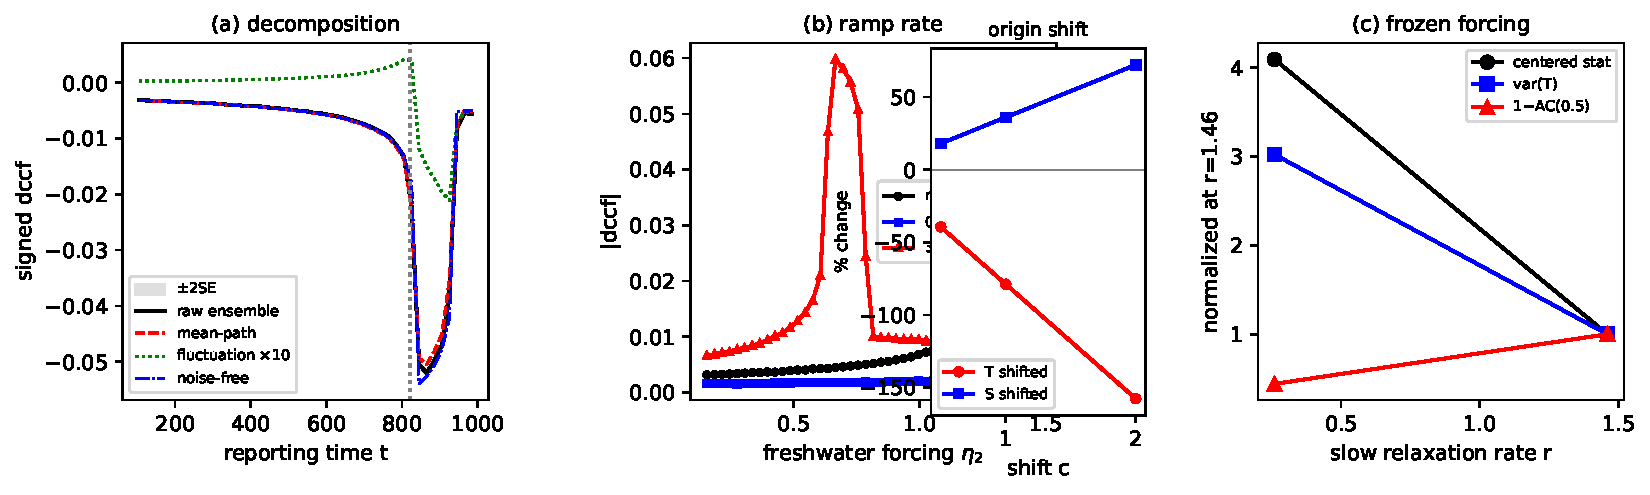
\includegraphics[width=\textwidth]{figures/fig6_stommel.pdf}
\caption{Drift in the irreversibility indicator of Ref.~\cite{kooloth2026} for the ramped Stommel model; data regenerated with the generation code of the authors' notebook~\cite{koolothcode2025}, adding only seeds. (a) Signed statistic against reporting time: raw ensemble mean and its mean-path, fluctuation and cross terms, and the value on the noise-free trajectory; bands, $\pm2$ standard errors. (b) Left, the original statistic against $\eta_2$ for three ramp rates; right, its relative change when $T$ or $S$ is shifted by $c=0.5$, 1 and 2. (c) Frozen forcing: centered statistic, variance of $T$ and $1-$AC1 against the slow relaxation rate $r$, each normalized at $r=1$.}
\label{fig:stommel}
\end{figure*}
